\documentclass{article}\usepackage[]{graphicx}\usepackage[]{color}
%% maxwidth is the original width if it is less than linewidth
%% otherwise use linewidth (to make sure the graphics do not exceed the margin)
\makeatletter
\def\maxwidth{ %
  \ifdim\Gin@nat@width>\linewidth
    \linewidth
  \else
    \Gin@nat@width
  \fi
}
\makeatother

\definecolor{fgcolor}{rgb}{0.345, 0.345, 0.345}
\newcommand{\hlnum}[1]{\textcolor[rgb]{0.686,0.059,0.569}{#1}}%
\newcommand{\hlstr}[1]{\textcolor[rgb]{0.192,0.494,0.8}{#1}}%
\newcommand{\hlcom}[1]{\textcolor[rgb]{0.678,0.584,0.686}{\textit{#1}}}%
\newcommand{\hlopt}[1]{\textcolor[rgb]{0,0,0}{#1}}%
\newcommand{\hlstd}[1]{\textcolor[rgb]{0.345,0.345,0.345}{#1}}%
\newcommand{\hlkwa}[1]{\textcolor[rgb]{0.161,0.373,0.58}{\textbf{#1}}}%
\newcommand{\hlkwb}[1]{\textcolor[rgb]{0.69,0.353,0.396}{#1}}%
\newcommand{\hlkwc}[1]{\textcolor[rgb]{0.333,0.667,0.333}{#1}}%
\newcommand{\hlkwd}[1]{\textcolor[rgb]{0.737,0.353,0.396}{\textbf{#1}}}%
\let\hlipl\hlkwb

\usepackage{framed}
\makeatletter
\newenvironment{kframe}{%
 \def\at@end@of@kframe{}%
 \ifinner\ifhmode%
  \def\at@end@of@kframe{\end{minipage}}%
  \begin{minipage}{\columnwidth}%
 \fi\fi%
 \def\FrameCommand##1{\hskip\@totalleftmargin \hskip-\fboxsep
 \colorbox{shadecolor}{##1}\hskip-\fboxsep
     % There is no \\@totalrightmargin, so:
     \hskip-\linewidth \hskip-\@totalleftmargin \hskip\columnwidth}%
 \MakeFramed {\advance\hsize-\width
   \@totalleftmargin\z@ \linewidth\hsize
   \@setminipage}}%
 {\par\unskip\endMakeFramed%
 \at@end@of@kframe}
\makeatother

\definecolor{shadecolor}{rgb}{.97, .97, .97}
\definecolor{messagecolor}{rgb}{0, 0, 0}
\definecolor{warningcolor}{rgb}{1, 0, 1}
\definecolor{errorcolor}{rgb}{1, 0, 0}
\newenvironment{knitrout}{}{} % an empty environment to be redefined in TeX

\usepackage{alltt}
\IfFileExists{upquote.sty}{\usepackage{upquote}}{}
\begin{document}

\title{Unemployment and its Educational Predictors}
\author{
Alcorn, Bryan\\
Shane, Joelle\\
Vogel, Abby\\
Vogel, Todd\\
}
\date{\today}

\maketitle

\begin{abstract}
In this research we look into the efficacy of secondary education on post graduation unemployment as well as whether public spending is effective at improving the quality of education.  To do this we utilized 3 predictive models (ridge, lasso, and pcr) and hypothesis testing.
\end{abstract}
\maketitle
\section{Introduction}

According to the US Bureau of Labor Statistics, those with a Bachelor's Degree have nearly twice the weekly earnings of those who have only a High School Degree (2006 Data). With the cost of education rising, it is ever important to be sure that the college a student choses attend will equipt them to have a career that can pay back their student loans. 

The College Scorecard ia a source of reliable nationwide data on over 7,000 institutions. This site, collegescorecard.gov, is a project of the Department of Education to aggregate annual data on higher education institutions. It has information from 19 years assembled from numerous sources. More information on the data can be found at collegescorecard.gov/data. 

The goal of this data was to create a resource for students, parents, and counsellors to be able to access information about the preformance of colleges and universities, and compare which school is the best fit. President Obama announced the New College Scorecard in September of 2015 as a means for people to better find an affordable and reputable institution to prepare themselves to enter the workforce. 

The goal of this analysis is to determine the features of institutions that lead to high employment rates post-graduation in order to answer the research question: does public spending improve the quality of education? We assume that employment after graduation is an accurate reflection of the quality of education the students recieve at a particular school. By focusing on public spending through data on financial aid reciepients, in conjunciton with other predictor variables, this analysis will reveal the ways in which public spending can impact the quality of a post-secondary schooling. This analysis could also be used by schools that wish to increase their post-graduation employment rates.
\maketitle
\section{Data}

This analysis uses data from 2006. The 2006 data was selected because it contains the unemployment rate via Census Data, which was selected to be the response variable. Unemplyment rate was chosen as the response variable because it is a robust measure across different sized and located institutions.

To clean the data, all factor variables were changed to numeric. Each variable with more than 50\% null values was removed. The remaining missing values were replaced by the median of the variable. Data was both mean-centered and standardized.

Two data sets were created for the modeling. First, the full cleaned data with over 500 variables was used. Initially, Principle Component Analysis was used to reduce the number of variables, but resulted in all variables in the first component. Because of this, the full cleaned data was used in the model.

In addition, a reduced set of predictor variables were selected from the full data by their perceived importance in educational success. This shortened data set was pulled from the data before the greater than 50\% NA variables were removed. 

The shortened data includes:

\begin{itemize}
\item Unemployment Rate (as response variable)
\item Instructional expenditures per full-time equivalent student
\item In-state tuition and fees
\item Average faculty salary
\item Completion rate for first-time, full-time students at four-year institutions (150\% of expected time to completion/6 years)
\item Completion rate for first-time, full-time students at less-than-four-year institutions (150\% of expected time to completion)
\item First-time, full-time student retention rate at four-year institutions
\item Percent of students who received a Pell Grant at the institution and who completed in 2 years at original institution
\item Percent of students who received a Pell Grant at the institution and who completed in 3 years at original institution
\item Percent of students who received a Pell Grant at the institution and who completed in 4 years at original institution
\item Two-year cohort default rate
\end{itemize}

Other variables were considered, but many weren't available in the 2006 data. 

Further analysis across years would provide a better look into weather or not a change in spending impacts the post-graduation unemployment rate, but was beyond the scope of the data available via The College Scorecard. 

\maketitle
\section{Methods}

This project involved the use and implementation of 3 different linear models as well as hypothesis testing.

\subsection{Ridge Regression}

Ridge Regression is the first of the two shrinkage modelling methods we used.  When using shrinkage methods the goal is to penalize certain parameters that should have a less significant effect on the model. To do so we use the tuning parameter, $\lambda$, times $\sum_{j=1}^{p}\beta_{j}^{2}$ to yield the shrinkage penalty. We then determine the coefficients that minimize the following equation:

\begin{equation}
\sum_{i=1}^{n}(y_i-\beta_0-\sum_{j=1}^{p}\beta_jx_{ij}) + \lambda\sum_{j=1}^{p}\beta_{j}^{2}
\end{equation}

To find these coefficients we used the function $cv.glmnet()$ to determine through cross validation which $\lambda$ value minimizes the above function (when $\lambda$ was a given sequence of numbers under $grid$, and $alpha$ was set to 0). From there we calculated the mean squared error (a measure of predicted power), by using the function:

\begin{equation}
MSE = \frac{1}{n}\sum_{i=1}^{n}(y_i - y_{di})^2
\end{equation}

\subsection{Lasso Regression}

Lasso regression is the second and final shrinkage modelling method used in this project. Although it is very similar to ridge regression there are a few key differences: the shrinkage penalty is now $\lambda$, times $\sum_{j=1}^{p}\beta_{j}^{2}$ ($\beta$ is not squared), and lasso allows for the removal of certain variables (not just dampening their effect). To determine the coefficients we must look for the $\beta$'s that minimize:

\begin{equation}
\sum_{i=1}^{n}(y_i-\beta_0-\sum_{j=1}^{p}\beta_jx_{ij}) + \lambda\sum_{j=1}^{p}|\beta_{j}|
\end{equation}

Again, to find the coefficient we used $cv.glmnet()$ and set $\lambda$ to $grid$. However, now, $alpha$ was set to 1. Finally, we calculated MSE to determine the predictive power of our model.

\subsection{Principle Components Regression}

PCR is the first of two dimension reduction modelling methods we used.  This method labors under the assumption that a subset of all of the predictor variables account for the vast majority of the variance.  These more significant variables are referred to as principle components (M).  PCR works by setting M equal to some reduced number of variables and running cross validation on, the model with the lowest cross validation error is selected.

To develop a model through PCR we used the $pcr()$ function and set $validation$= CV.  We then found the model in which PRESS was larger to avoid overfitting. Finally, we calculated MSE to determine the predictive power of our model.

\subsection{Hypothesis Testing}

Hypothesis tests allows for comparison across groups. By separating the data points into categories based on how much funding the school received, we can then compare those categories based on unemployment rate and see how they differ.


To utilize this method we:
\begin{itemize}
\item Separated the data into groups by amount of funding the school received (low, low-mid, mid-high, high). 
\item Created hypothesis test, $W(u)$, to describe the difference being analyzed.
\item Computed the estimate for effect of funding and variance of that effect.
\end{itemize}

\maketitle
\section{Analysis}

\subsection{Modelling}
In the Results section of the report, we determined the mean squared error values for each of our 3 models (one model with every variable from the data included and one where we preselected 10 variables).  For the full Ridge, Lasso, and PCR the MSE's were 0.186, 0.195, and 0.271 respectively. For the shor Ridge, Lasso, and PCR the MSE's were 12.797, 17.114, and 1.446 respectively. Because our data was mean centered and standardized, all of these values exist on the same scale and can thus be prepared.  Mean squared error values represent the average sum of the errors between actual and predicted response values. Therefore, the smaller the MSE value the smaller the error, and the better the predictive model.  Given this, 0.186 is our smallest MSE value meaning Ridge is our best predictive model. These results are unsurprising to an extent, each of the MSE's for the shortened models were much higher, meaning that preselecting predictors negatively effects the modelling process.  

In order to determine which variables most affected unemployment rates we look at the absolute values of the coefficients from our best model (ridge) and look at the top 5. 


% latex table generated in R 3.3.2 by xtable 1.8-2 package
% Mon Dec  5 17:55:29 2016
\begin{table}[ht]
\centering
\begin{tabular}{rlr}
  \hline
 & Predictor & Coefficient \\ 
  \hline
1 & POVERTY\_RATE & 0.71 \\ 
  2 & PCT\_WHITE & -0.42 \\ 
  3 & PCT\_BA & -0.18 \\ 
  4 & PCT\_BLACK & -0.14 \\ 
  5 & PCT25\_EARN\_WNE\_P6 & -0.11 \\ 
   \hline
\end{tabular}
\caption{Information about top 5  Ridge Model Coefficients} 
\end{table}


This result means that the 5 most important predictors of unemployment rate are poverty rate, \% white, \% bachelors degrees given (of total degrees given), \% black, and married.  Schools with higher poverty rates have higher unemployment after graduation, wheres the schools with higher values of the other 4 variables with have lower rates of unemployment.

\subsection{Hypothesis Testing}
The estimate for the effect of spending on quality of education recieved was about -5.4\%. This means every higher spending bracket is expected to have a 5.4\% increase in unemployment. The variance on this value was about 0.0025, making it significant. After separating the data by average faculty salary, we can see that unemployment was the highest among schools that had low average faculty salary and the lowest among schools taht had high average faculty salary. We still estimate that higher spending is associated with higher unemployment, but since controlling for just a single factor showed a decrease in the effect, we could expect continual descreases or even a reversal of the effect if we continued to control for more and more variables.
\maketitle
\section{Results}

\subsection{Modeling}
After forming the aforementioned regression models we found 10 coefficients that represent the best fit for each model. The resulting predictive function looks like:

\begin{equation}
Y = \beta_0 + \beta_1 X_1 + \beta_2 X_2 + \beta_3 X_3 + \beta_4 X_4 + \beta_5 X_5 + \beta_6 X_6 + \beta_7 X_7 + \beta_8 X_8 + \beta_9 X_9 + \beta_{10} X_{10}
\end{equation}



\begin{center}
\begin{table}[ht]
\centering
\caption{Information about Model Coefficients} 
\begin{tabular}{rlrrr}
  \hline
 & Variables & Ridge & Lasso & PCR \\ 
  \hline
1 & UNEMP\_RATE & 0.000 & 0.000 & 0.000 \\ 
  2 & INEXPFTE & 0.000 & -0.000 & -0.008 \\ 
  3 & TUITIONFEE\_IN & -0.963 & -0.156 & -0.182 \\ 
  4 & AVGFACSAL & -0.786 & -0.067 & -0.089 \\ 
  5 & C150\_4 & -0.695 & -0.119 & -0.123 \\ 
  6 & C150\_L4 & 0.594 & 0.000 & 0.002 \\ 
  7 & RET\_FT4 & 0.978 & 0.000 & 0.027 \\ 
  8 & PELL\_COMP\_ORIG\_YR2\_RT & -2.752 & 0.000 & -0.111 \\ 
  9 & PELL\_COMP\_ORIG\_YR3\_RT & 0.491 & 0.042 & 0.125 \\ 
  10 & PELL\_COMP\_ORIG\_YR4\_RT & 1.372 & 0.000 & 0.020 \\ 
  11 & CDR2 & 0.498 & 0.120 & 0.166 \\ 
   \hline
\end{tabular}
\end{table}

\end{center}

This table presents the fit between the prediction variables and the response variable ($Unemployment$) determined from the $cv.glmnet()$ and $pcr()$ functions, for each of our 3 models (Ridge, Lasso, PCR).

After finding the 5 predictive functions, we found the MSE's for each model:

\begin{center}

\begin{table}[ht]
\centering
\caption{Information about Mean Squared Errors} 
\begin{tabular}{rlr}
  \hline
 & Model & MSE \\ 
  \hline
1 & Ridge & 0.184 \\ 
  2 & Short Ridge & 12.797 \\ 
  3 & Lasso & 0.193 \\ 
  4 & Short Lasso & 17.114 \\ 
  5 & PCR & 0.278 \\ 
  6 & Short PCR & 1.446 \\ 
   \hline
\end{tabular}
\end{table}


\end{center}


Analysis of these numbers will reveal which model has the most predictive power.

\subsection{Hypothesis Testing}

For hypothesis testing method unemployment rate was set as our response variable and school funding was set as the independent variable (percent of students recieving financial aid).

If the amount of funding received by the school has no effect on quality of education rate, we should see little difference in the response variable (unemployment rate), and that difference is solely due to chance.


\graphicspath{ {../images/} }
\begin{figure}
\centering
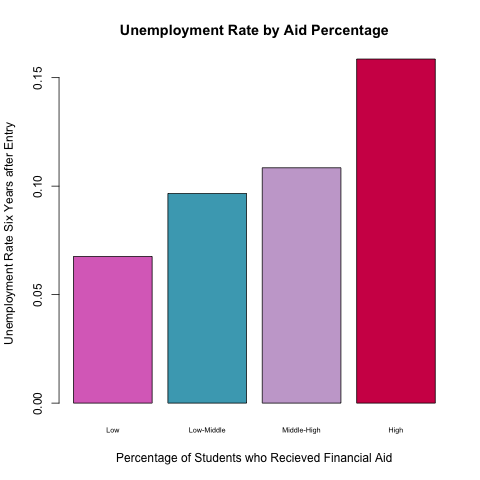
\includegraphics[width=0.5\textwidth]{unemployment}
\caption{Effect of spending on unemployment rate}
\end{figure}



We looked for estimate (of effect of spending on unemployment). This value will reveal the relationship between our two variables.  A higher estimate means that spending has a significant effect on unemployment and a negative estimate means that spending has an inverse effect on unemployment.

Estimate of effect of spending on unemployment rate:
\begin{knitrout}
\definecolor{shadecolor}{rgb}{0.969, 0.969, 0.969}\color{fgcolor}\begin{kframe}
\begin{verbatim}
## [1] -0.05141263
\end{verbatim}
\end{kframe}
\end{knitrout}

To control for a difference in unemployment rate generated from the difference in faculty quality, the data was split into three groups, corresponding to schools that had low, medium, and high average faculty salary.  


\graphicspath{ {../images/} }
\begin{figure}
\centering
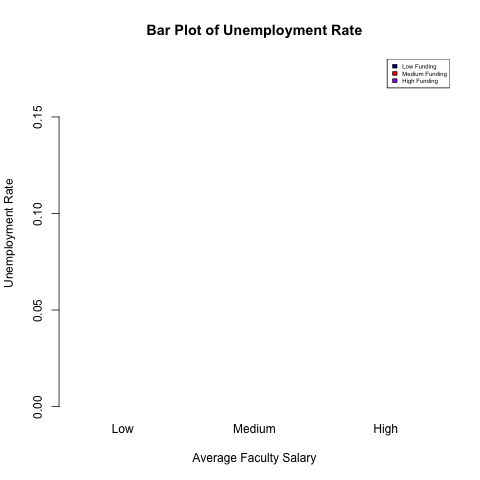
\includegraphics[width=0.5\textwidth]{funding}
\caption{Effect of spending on unemployment rate, controlling for quality of teachers}
\end{figure}


While the results still show that more spending is associated with more unemployment, we can see that average faculty salaray did influcence unemployment rate, as schools that have higher average faculty salary also had a lower unemployment rate, in general. 

Estimate of the effect of spending on unemployment rate (low average faulty salary):
\begin{knitrout}
\definecolor{shadecolor}{rgb}{0.969, 0.969, 0.969}\color{fgcolor}\begin{kframe}
\begin{verbatim}
## [1] -0.07196604
\end{verbatim}
\end{kframe}
\end{knitrout}

Estimate of the effect of spending on unemployment rate (middle average faulty salary):
\begin{knitrout}
\definecolor{shadecolor}{rgb}{0.969, 0.969, 0.969}\color{fgcolor}\begin{kframe}
\begin{verbatim}
## [1] -0.08068517
\end{verbatim}
\end{kframe}
\end{knitrout}


Estimate of the effect of spending on unemployment rate (high average faulty salary):
\begin{knitrout}
\definecolor{shadecolor}{rgb}{0.969, 0.969, 0.969}\color{fgcolor}\begin{kframe}
\begin{verbatim}
## [1] -0.06582947
\end{verbatim}
\end{kframe}
\end{knitrout}
\maketitle
\section{Conclusion}

From hypothesis testing, we found public spending negatively effected unemployment rate; schools that recieved more funding provided lower quality educations. These results are difficult to justify, given how many confounding factors there could be in the data. After trying to control for school quality the effect was less negative but still significant. To try and find predictors of unemployment rate, which would allow educational institutions to improve unemployment rate independent of the public spending they received, we ran a few different regression models. When predictors of unemployment rate were manually selected for the regression models, the mean squared error was much larger than when predictor variables were selected through dimension reduction methods. 

\maketitle
\section{Appendix}

\subsection{Additional Information and thoughts about this project - Further reading}

We originally wanted to include funding in our research model. 

While we could not completely answer the research question, hopefully this project gave a better idea of how certain variables might contribute to the success of certain decisions. As students, we are concerned with how decisions are made about how to distribute resources towards bettering education. Since we were missing a lot of data and not able to compare over the years for change, we could not completely answer how to make the best decision to better educational success. 

\subsection{Further Possibilities}
Hopefully important decisions are made with data like this. We developed a project as a guide for further analysis. With more data and analysis, we would like to analyze the best predictor of how to actually tell what indicates the success of an institution. We went through some of the post graduation data by hand and thought unemployment is a good indicator, but probably not the best. We learned from our short models that hand selecting data does not produce the best results. A better predictor of an institution's success is probably a combinations of factors, not just one.

Another further step would be more complicated algorithms. One idea we had was running a machine learning algorithm such as a neural net to try and classify the data into certain levels such as needs improvement all the way to highly successful institutions. Running this would tell help us classify new institutions as either successful or not as well as telling us what variables would make the university better. The idea behind this is maximum effect for the added effort. The reason this is superior to our linear models is it actually classifies the data. Instead of just predicting what the unemployment rate might be with a certain combination of variables, we would instead be able to classify and make judgements. 

\subsection{Problems and shortcomings}
Hand selecting data is not an ideal statistical approach, but we did it to see if we could predict about as accurately with only a limited number of variables. We hand selected these variables because we wanted to see if things we intuitively thought were relative would actually be useful predictors. Turns out there are hiding factors that contribute more to unemployment in institutions than we thought. Again, this indicates how important further testing should be done for better decision making. 

After we hand selected what we thought were pertinent variables, we were disappointed to learn that many were mostly null in the year we selected, another shortcoming indicating how important data is to better results. 

What is a key variable? Key variables defined as ones that we think may indicate a successful university in that they will have a low unemployment rate. These are things we care about and want to compare across schools. If we can say something like in state tuition has x weight it is more helpful than comparing one of the more specific variables

We initially thought PCA would be helpful in grouping data into components so we could find a subset of the data that was more important to the data. Unfortunately, with this many variables, we were only able to put them all in one component making that plan pointless. 



\end{document}
